% vim: spell spl=pt fo+=tcaw tw=78 nonu sw=4 ts=4
% vim: fen fdc=1 fdm=marker fmr={{{,}}}

% sbc {{{
\documentclass[12pt]{article}
% }}}
% abnt {{{
%\documentclass{abnt}
% }}}
% packages {{{
\usepackage[brazil]{babel}
\usepackage[utf8]{inputenc}
\usepackage[T1]{fontenc}
\usepackage{graphicx}
\usepackage{epstopdf}
%\usepackage{wrapfig}
%\usepackage{caption}
\usepackage{float}
\usepackage{url}
\usepackage[bookmarks]{hyperref}
% }}}
% sbc {{{
\usepackage{sbc-template}
%}}}
% abnt {{{
%\usepackage[num]{abntcite}
% }}}
     
\sloppy

% sbc {{{
\title{Transições Interrede Independentes do Meio Físico de Acesso}
\author{Higor Eurípedes P. F. A.\inst{1}, Cláudio de C. Monteiro\inst{1}}
\address{Instituto Federal de Educação, Ciência e Tecnologia do Tocantins 
	(IFTO)\\
  77.021-090 -- Palmas -- TO -- Brazil
  \email{heuripedes@gmail.com, ccm@ifto.edu.br}
}
\date{Março, 2012}
% }}}
% abnt {{{
%\titulo{Transições Interrede Independentes do Meio Físico de Acesso}
%\autor{Higor Eurípedes P. F. A.}
%\orientador{Cláudio de C. Monteiro}
%\instituicao{Instituto Federal de Educação, Ciência e Tecnologia do Tocantins}
%\local{Palmas -- TO -- Brasil}
%\data{Fevereiro, 2012}
% }}}

\begin{document}

% sbc {{{
\maketitle
% }}}
% abnt {{{
%\capa
%\folhaderosto
%\sumario
% }}}

\begin{resumo}

Com o surgimento dos dispositivos multi interface, tornou possível o acesso 
ininterrupto a serviços, porém a estrutura lógica em uso se mostrou 
despreparada para esta nova demanda.

Este artigo, apresenta o padrão IEEE 802.21 de transições independentes do 
meio e propõe uma implementação distribuída baseada num subconjunto dos 
conceitos do mesmo.

\end{resumo}

\begin{abstract}

The emerging multi-interface device market, has made possible the seamless 
access to services based on general purpose networks, but the logic structure 
of the in-use techniques has proved unprepared to this new demand.

This paper, introduces the IEEE 802.21 standard for media independent handover 
and proposes a distributed implementation based on a subset of the concepts 
presented on the said standard.

\end{abstract}

% abnt {{{
%\chapter{Introdução}
% }}}

\section{Introdução} \label{sec:introducao} % {{{

A crescente procura por mobilidade impulsionou a venda de dispositivos móveis.  
Cada vez mais exigentes, os usuários demandam do mercado dispositivos que os 
permitam proceder com suas atividades onde e como lhe convir. Estas pessoas, 
em geral, gastam boa parte de seu dia utilizando ferramentas dependentes da 
\textit{internet} e, portanto, precisam de soluções que lhes permitam gozar da 
portabilidade de seus dispositivos ao realizar estas atividades.

Para atender esta demanda, tecnologias de comunicação sem fio como 
\textit{WiFi} (IEEE 802.11 \cite{ieee:2007:80211}), \textit{WiMAX}
(IEEE 802.16\cite{ieee:2009:80216}) e 3g (\textit{3GPP} e \textit{3GPP2}) 
foram desenvolvidas.  Entretanto, a evolução dos dispositivos móveis 
introduziu o conceito de multiacesso (capacidade de se conectar a mais de uma 
rede ou tipo de rede simultaneamente), uma característica que tornou evidente 
uma deficiência da infraestrutura atual: a transição entre redes é incômoda e 
causa quedas de disponibilidade de certos serviços.  Segundo \cite{piri:2009}, 
isto acontecia, parcialmente, por falta de padronização dos mecanismos de 
transição em uso.  Para sanar estas deficiências, deu-se inicio ao 
desenvolvimento de um novo padrão aberto para a transição interrede 
independente do meio físico de acesso: o padrão IEEE 802.21 
\cite{ieee:2008:80221}, intitulado \textit{Media Independent Handover 
Services}.

O padrão IEEE 802.21 documenta mecanismos auxiliares para transição entre 
redes heterogêneas. O objetivo principal é facilitar o processo de 
\textit{handover} por meio de uma abstração das camadas inferiores chamada 
\textit{Media Independent Handover Function} (MIHF). Esta camada é basicamente 
composta de serviços independentes do meio que permitem comunicação entre 
\textit{MIH Users} e entre camadas.

Nas quatro seções seguintes, estão presentes a justificativa, a problemática, 
os objetivos e a metodologia utilizada nesta pesquisa, respectivamente. A 
seção seção 6 apresenta uma visão geral do padrão, e em seguida são 
apresentados os detalhes de uma proposta de implementação do mesmo.
%}}}

\section{Funcionamento do padrão IEEE 802.21} \label{sec:padrao} % {{{

\subsection{A MIHF}

O padrão IEEE 802.21 documenta mecanismos que auxiliam a transição entre redes 
heterogêneas.  Em \cite{idigital:2009}, o padrão é caracterizado como uma 
abstração da camada de enlace, oferecendo às camadas superiores um acesso 
comum independente da tecnologia de enlace empregada.

É mencionado em \cite{ieee:2008:80221}, que o objetivo principal do padrão é 
facilitar o processo de transição entre redes IEEE 802 - tornando-o 
independente do meio de transmissão utilizado - e permitir a conectividade 
ininterrupta dos dispositivos garantindo uma experiência de continuidade de 
conexão para o usuário.  Embora tenha foco na transição entre redes IEEE 802 
heterogêneas, o padrão também poderá ter seus mecanismos utilizados para 
efetuar transições homogêneas ou entre redes IEEE 802 e redes não-IEEE 802.  

Para \cite{piri:2009}, o elemento principal do padrão é a \textit{Media 
Independent Handover Function} (MIHF). Esta função é uma entidade lógica, 
localizada entre as camadas 2 e 3, que tem a tarefa de assistir transições dos 
\textit{Mobile Nodes} (MN), dispositivos com capacidade para acessar várias 
redes simultâneamente. Em \cite{kimhun:2010}, é afirmado que a MIHF oferece 
uma abstração das camadas inferiores sob a forma de interface unificada, 
visando assistir as aplicações das camadas superiores durante o processo de 
\textit{handover}. Esta interface é composta de três serviços disponibilizados 
aos nós da rede:

\begin{enumerate}

	\item \textit{Media Independent Event Service} (MIES) -- fornece 
	classificação, filtragem e notificação de eventos correspondentes à 
	alterações das propriedades das camadas inferiores. O serviço também é 
	capaz notificar as camadas superiores de eventos que irão ocorrer.

	\item \textit{Media Independent Command Service} (MICS) -- permite que 
	camadas superiores sejam capazes de reconfigurar ou selecionar 
	conexões por meio de comandos de transição.

	\item \textit{Media Independente Information Service} (MIIS) --  
	fornece detalhes sobre serviços disponíveis na rede atual e nas 
	vizinhas.
	
\end{enumerate}

A transmissão e recepção de comandos, eventos e informações entre os serviços 
e os clientes MIH, são feitos utilizando o protocolo \textit{Media Independent 
Handover Protocol} (MIHP). Segundo \cite{ieee:2008:80221}, este protocolo 
permite a troca de mensagens MIH entre as MIHFs das entidades ao nível das 
camadas dois e três. A comunicação pode ser feita de forma síncrona ou 
assíncrona, utilizando pares de requisição e resposta ou o método 
\textit{push}, onde uma MIHF envia uma mensagem à outra mesmo sem solicitação.

%O IEEE 802.21 foi criado para abranger tanto tecnologias IEEE quanto 
%tecnologias não-IEEE. Segundo \cite{taniuchi:2009}, o padrão possibilita o 
%\textit{handover} vertical criando-se uma única extensão (MIH\_LINK\_SAP) 
%para cada tecnologia envolvida, porém este objetivo nobre pode ser difícil de 
%se alcançar à curto prazo por culpa da quantidade de padrões e tecnologias 
%dentro e fora dos domínios da IEEE.

%}}}

\subsection{As transições} % {{{

Como apresentado anteriormente, o padrão 802.21 possui foco nas transições 
verticais, isto é, transições entre redes heterogêneas. Estas transições são 
realizadas de modo a garantir um uso otimizado dos recursos da rede e dos 
dispositivos, além de promover a continuidade dos serviços oferecidos aos 
usuários.

Transições que obedecem o padrão IEEE 802.21 podem ser motivadas por eventos 
propagados pelo MIES ou por comandos enviados ao MICS. O MIIS fica responsável 
por disponibilizar às camadas superiores informações suficientes sobre a 
situação da rede alvo, de modo a permitir a escolha que apresente menor custo.  
Detalhes específicos sobre os procedimentos da operação ficam sob a 
responsabilidade do fornecedor, segundo \cite{stein:2006}.

Para exemplificar o trabalho dos serviços durante um \textit{handover}, 
pode-se considerar a seguinte situação adaptada de \cite{kimhun:2010}: 

\begin{enumerate}

	\item Um determinado local é coberto por duas redes, uma WiFi (rede A) 
	e outra WiMAX (rede B), e, no momento, existem alguns dispositivos 
	clientes (C) conectados à rede A;

	\item O administrador da rede A decide efetuar a manutenção no único 
	\textit{access point} (\textit{Point of Attachment} ou PoA) da rede e, 
	utilizando um programa de gerência com suporte a MIH e MICS, envia à 
	MIHF de seus clientes uma \textit{MIH\_Net\_HO\_Candidate\_Query 
	request} para iniciar a transição e sugerir pontos de acesso 
	alternativos. Os clientes respondem com uma 
	\textit{MIH\_Net\_HO\_Candidate\_Query response} informando os pontos 
	de acesso  e conexões preferidas;

	\item O PoA da rede A solicita informações adicionais aos MIIS dos 
	PoAs sugeridos pelo cliente por meio de uma 
	\textit{MIH\_N2N\_HO\_Query\_Resource request}, e os mesmos respondem 
	com uma \textit{MIH\_N2N\_HO\_Query\_Resource response}. Com esta 
	informação o PoA atual determina qual PoA receberá os clientes, no 
	caso, o PoA da rede B.

	\item Uma \textit{MIH\_Net\_HO\_Commit request} contendo o PoA de destino 
	é enviada aos clientes para que efetuem a transição. O PoA atual 
	notifica os PoAs vizinhos que a transição irá ocorrer utilizando uma 
	\textit{MIH\_N2N\_HO\_Commit request} que informa qual cliente e quais 
	PoAs estão envolvidos. Os clientes e o PoA alvo ao concluirem a 
	operação de \textit{handover} respondem ao PoA inicial com uma 
	\textit{MIH\_Net\_HO\_Commit response} e \textit{MIH\_N2N\_HO\_Commit 
	response}, respectivamente.

\end{enumerate}

A situação mais comum, vivida em ambientes que implementam MIH, é a que ocorre 
sem intervenção, por meio de eventos propagados pelo MIES dos MN. Tomando o 
exemplo anterior como ponto de partida, pode-se substituir a intervenção do 
administrador de redes pela degradação de sinal, causada pela movimentação do 
dispositivo. Neste momento, o MIES do cliente dispara o evento 
\textit{MIH\_Link\_Going\_Down} para que o PoA associado solicite informações 
do estado dos PoAs adjacentes.
% }}}

\section{Trabalhos relacionados} \label{sec:proposta}

%Esta seção discute sobre algumas escolhas feitas nas obras de 
%\cite{tawil:2008}, \cite{kimhun:2010}, \cite{machan:2008} e 
%\cite{taniuchi:2009}. 

%ESQUEMA DISTRIBUÍDO

%A decisão de \textit{handover}

O trabalho de \cite{tawil:2008}, analisa o comportamento de um processo 
distribuído de transição, o que é justificado por permitir que os elementos 
envolvidos sejam capazes de tomar decisões mais realistas em relação ao 
ambiente.  Isso é possível graças à participação ativa de estações servidoras 
no processo de decisão.

Estas decisões realísticas, possibilitam a economia de recursos computacionais 
e uma experiência aprimorada.  Resultados apresentados em \cite{tawil:2008}, 
comprovam a superioridade deste modelo, em termos de rendimento de 
rede\footnote{O rendimento de rede é inversamente proporcional à quantidade de 
pacotes perdidos durante o processo de \textit{handover}.} e tempo de 
processamento de decisões\footnote{O tempo ou atraso de processamento de 
decisão, significa quanto tempo o sistema demorou para processar as 
informações de \textit{handover} e tomar uma decisão.} (figuras 
\ref{fig:dvhds-throughput} e \ref{fig:dvhds-procdelay}), em relação aos 
esquemas centralizados. Seu esquema utiliza NQVs\footnote{O Valor de Qualidade 
de Rede é calculado levando em consideração itens como largura de banda, 
segurança, custo monetário e consumo de energia.} para determinar a rede mais 
benéfica ao usuário. 

\begin{figure}[ht]
	\centering
	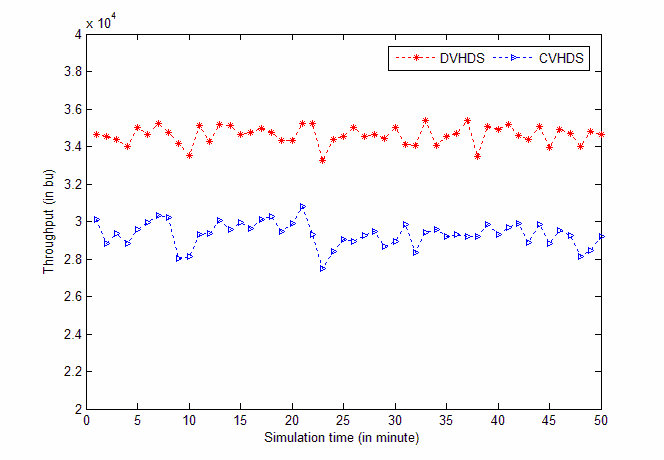
\includegraphics[width=.8\textwidth]{pre-projeto/dvhds-throughput.png}
	\caption{Rendimento de rede (em unid. de largura de banda) ao longo do 
	tempo (\cite{tawil:2008}).}
	\label{fig:dvhds-throughput}
\end{figure}

\begin{figure}[ht]
	\centering
	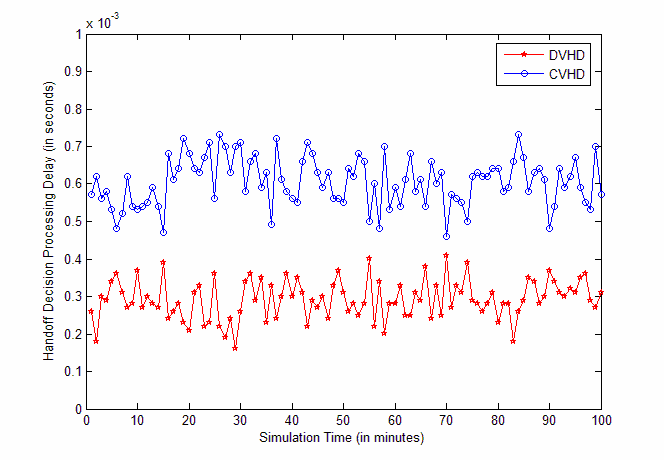
\includegraphics[width=.8\textwidth]{pre-projeto/dvhds-procdelay.png}
	\caption{Tempo de processamento (em segundos) ao longo do tempo 
	(\cite{tawil:2008}).}
	\label{fig:dvhds-procdelay}
\end{figure}

% PRIMITIVAS


% ESQUEMA DE TAWIL, LADO RUIM DA ESCOLHA DEPENDENTE DE POAs

% MELHORAR ESTE PARAGRAFO vvvvvvvvvvvvvvvvvvvvvvvvvvvvvvvvvvvvvvvvvvvvvvvvvv

Outro fator que pode influenciar na eficiência do esquema são as primitivas 
utilizadas.  O evento MIH\_Link\_Going\_Down\footnote{O evento 	
MIH\_Link\_Going\_Down é disparado pelo MIES quando o mesmo é notificado pelo 
MIH\_LINK\_SAP de que as condições do enlace estão se degradando e que ele 
poderá cair em breve.  (\cite{ieee:2008:80221})}, por exemplo,  pode passar 
despercebido aos olhos do pesquisador, contudo este evento proporciona 
melhoras de até 8\% no tempo de duração dos \textit{handovers}, segundo 
\cite{machan:2008} (Ver figura \ref{fig:machan}).  A quantidade de primitivas 
também pode influenciar na performance da solução, utilizar um número reduzido 
torna a passagem de mensagens menos flexível, porém mais concisa.

\begin{figure}[h!]
	\centering
	\includegraphics[width=.7\textwidth]{pre-projeto/machan.eps}
	\caption{Tempo de handover em relação à carga de rede.  
	(\cite{machan:2008})}
	\label{fig:machan}
\end{figure}

\begin{table}[h!]
	\centering
	\caption{Primitivas do esquema de \cite{tawil:2008}}
	\label{tab:tawil-primitivas}
	\begin{tabular}[b]{ l | l | l | l }
		Primitiva & Serviço & Padrão & Descrição \\
		\hline
		MIH\_Link\_Going\_Down   & MIES & Sim & O link poderá cair em breve. \\
		 MIH\_Handover\_Initiate & MICS & Não & Inicia o handover. \\
		MIH\_Get\_Status         & MICS & Não & Retorna o estado do link. \\
		MIH\_Switch              & MICS & Não & Efetua a troca entre links. \\
		MIH\_Get\_Information    & MIIS & Não & Solicita informações ao		
		repositório.\\
		\hline
	\end{tabular}
\end{table}

A tabela \ref{tab:tawil-primitivas} apresenta todas as primitivas utilizadas 
no esquema de \cite{tawil:2008}, nota-se a presença de quatro primitivas que 
não pertencem ao padrão. Estas primitivas são introduzidas para resumir e 
incrementar a funcionalidade das primitivas descritas no padrão.


\section{Justificativa} \label{sec:justificativa} % {{{

Seguindo a tendência atual, o futuro das aplicações domésticas, e de parte das 
industriais, está ligado à mobilidade oferecida pelo uso de serviços 
distribuídos e/ou de computação nas nuvens. Sejam eles para armazenamento e 
compartilhamento de arquivos, distribuição de conteúdo ou simplesmente acesso 
remoto a recursos.

Para garantir um futuro de continuidade e de qualidade de serviço, é preciso 
que a mobilidade seja levada além da existência da comunicação sem fio, é 
preciso integrar as tecnologias existentes de modo que o uso das redes se 
torne ubíquo.  É neste aspecto, que o IEEE 802.21 poderá se firmar como ponte 
entre tecnologias atuais e alicerce para as futuras..

% }}}
\section{Problemática} \label{sec:problematica} % {{{

Apesar da importância tecnológica, o padrão IEEE 802.21 ainda não é amplamente 
utilizado. Um dos fatores que impedem a adoção do padrão, é a resistência, 
justificada, que os operadores tem em relação a modificação de seus ambientes 
de rede; o segundo fator, foi o tempo que o padrão levou até chegar ao mercado 
e à academia.

Com isso em mente, este trabalho procura responder a seguinte pergunta: 
\textit{É possível reproduzir os mecanismos documentados no padrão IEEE 
802.21, de forma distribuída, num ambiente real?}
% }}}
\section{Objetivos} \label{sec:objetivos} % {{{

\subsection{Objetivos gerais}
Avaliar a viabilidade e as consequências da implantação de uma implementação 
de referência do padrão em um ambiente real.

\subsection{Objetivos específicos}

\begin{itemize}

	\item Estudar o funcionamento da MIHF;
	\item Propor uma arquitetura para a utilização da MIHF em ambientes reais;
	\item Implementar um subconjunto da funcionalidade do padrão:

		\begin{itemize}
	
			\item Descoberta de MIHFs;
			\item Notificação de eventos do link;
			\item Comandos para coleta de informação e para a realização das 
				transições.

		\end{itemize}

	\item Avaliar o desempenho da proposta, comparando com as soluções de 
		\cite{tawil:2008} e \cite{machan:2008}.
	
\end{itemize}
% }}}

\section{Metodologia} \label{sec:metodologia} % {{{

Para a realização desta pesquisa, será necessário realizar um estudo da 
bibliografia, a implementação de um subconjunto da \textit{Media Independent 
Handover Function} e a elaboração de um ambiente controlado para a realização 
de testes.  
%Ao término destes, será feita a coleta e analise quantitativa dos dados.

%% Perguntar ao Cláudio sobre esta 'análise quantitativa'


% }}}

\section{O esquema proposto}

A pesquisa se propõe a implementar um esquema distribuído de \textit{handover} 
baseado nas ideias discutidas anteriormente, em destaque no trabalho de 
\cite{kimhun:2010} e \cite{tawil:2008}. A avaliação da implementação será 
feita em um ambiente real e utilizará \textit{access points} (APs) como 
estações servidoras.

O ambiente é composto por duas redes, uma 3G e outra 802.11, e pelo menos uma 
estação móvel. A estação base da rede 802.11 e as estações móveis terão 
suporte às funcionalidades MIH, porém, assim como em \cite{taniuchi:2009}, a 
implementação não poderá contar com uma BS 3G que suporta MIH, pois não se tem 
acesso interno a esta rede.  Contudo, a BS da rede 802.11 poderá suprir 
informações sobre a rede celular, quando solicitada.

\begin{figure}[ht]
	\centering
	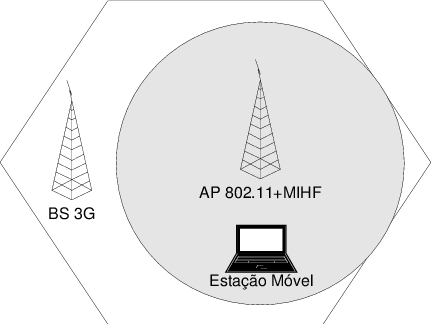
\includegraphics[width=.5\textwidth]{pre-projeto/ambiente.eps}
	\caption{Ambiente proposto.}
	\label{fig:ambiente}
\end{figure}

A MIHF utilizada poderá funcionar em modo servidor ou em modo cliente, a 
diferença reside no tratamento de requisições de descoberta: no modo cliente, 
requisições de descoberta são ignoradas, enquanto que no modo servidor as 
requisições deverão ser respondidas informando os links. Não será necessária a 
subscrição de eventos nem o cadastro junto às MIHFs servidoras, MIHFs que 
solicitarem informações a outras estarão automaticamente cadastradas e 
receberão notificações de eventos.

Assim como em \cite{tawil:2008}, o número de primitivas foi reduzido ao mínimo 
necessário para a implementação de notificação de eventos e transições.
Este conjunto contém eventos para lidar com mudanças de estado dos links, 
comandos para realização das transições e comandos para a obtenção de 
informações estáticas e dinâmicas. A tabela \ref{tab:primitivas}, contém uma 
relação de todas as primitivas que serão utilizadas. Na lista a seguir estão 
enumeradas as primitivas que foram introduzidas.  

\begin{enumerate}

	\item MIH\_Link\_Switch -- Esta primitiva é utilizada para realizar a 
		transição entre links. Substitui a funcionalidade das primitivas 
		MIH\_Net\_HO\_*, MIH\_N2N\_HO\_*, MIH\_MN\_HO\_* e 
		MIH\_Link\_Handover\_*.
	
	\item MIH\_Report -- Esta primitiva é utilizada para obter informações 
		sobre links presentes no ponto de acesso. Substitui a funcionalidade 
		das primitivas MIH\_Get\_Information, MIH\_Link\_Get\_Parameters e 
		MIH\_Link\_Parameters\_Report.
	
	\item MIH\_Discovery -- Esta primitiva é utilizada para descobrir
		pontos de acesso numa determinada rede. Uma requisição é enviada por 
		\textit{broadcast} ou \textit{multicast} e estações servidoras deverão 
		responder informando os links disponíveis. Estações cliente ignoram 
		estas requisições. Substitui a funcionalidade da primitiva
		MIH\_Register.

\end{enumerate}

\begin{table}
	\centering
	\caption{Primitivas do esquema proposto}
	\label{tab:primitivas}
	\begin{tabular}[ht]{ l | l | l }
		Primitiva & Serviço & Descrição \\
		\hline
		MIH\_Link\_Up          & MIES & O link está disponível. \\
		MIH\_Link\_Down        & MIES & O link está indisponível. \\
		MIH\_Link\_Going\_Down & MIES & O link poderá cair em breve. \\
		MIH\_Link\_Switch      & MICS & Realiza o \textit{handover}. \\
		MIH\_Report           & MICS & Obtém informações sobre uma estação. \\
		MIH\_Discovery   & MIIS & Procura MIHFs servidoras na rede.  \\
		\hline
	\end{tabular}
	
\end{table}

\begin{figure}[ht]
	\centering
	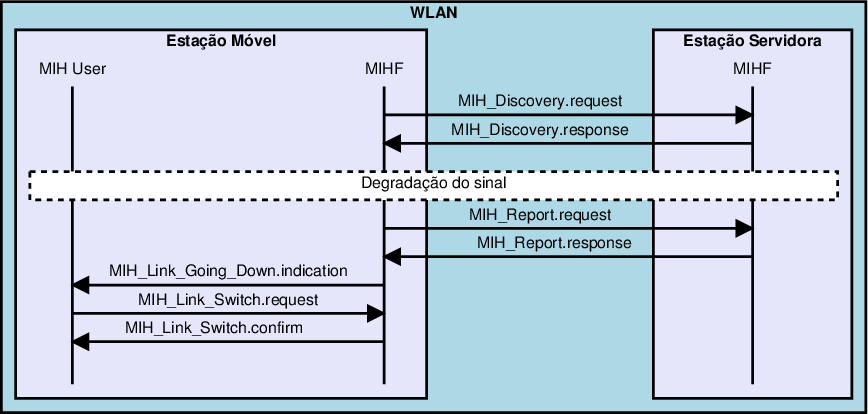
\includegraphics[width=\textwidth]{pre-projeto/novo-soft-handover.eps}
	\caption{Processo de \textit{soft-handover}.}
	\label{fig:soft-handover}
\end{figure}

A figura \ref{fig:soft-handover} demonstra a sequência de mensagens, desde a 
descoberta de MIHFs servidoras até o momento que ocorre um 
\textit{soft-handover}. Assim que recebe respostas à mensagem de descoberta, a 
MIHF da estação móvel envia mensagens MIH\_Report solicitando informações 
sobre redes que cobrem a região. O recebimento de um evento 
MIH\_Link\_Going\_Down, dispara o processo de transição e em seguida o usuário 
MIH solicita à MIH\_Link\_Sap que realize a troca entre links. No processo de 
\textit{hard-softover}, o evento MIH\_Link\_Down toma o lugar de 
MIH\_Link\_Going\_Down.

\section{Resultados esperados} \label{sec:esperados} % {{{

Espera-se avaliar a arquitetura proposta, usando uma implementação real, 
analisando sua eficiência em relação a continuação das conexões ativas do 
móvel, após sua migração entre redes.

%Como produto da pesquisa, espera-se que o esquema proposto seja viável e que 
%apresente um impacto positivo no ambiente onde será implantado. Seu 
%funcionamento, deverá ser de baixo impacto, porém ágil.

%}}}

\section{Conclusão} \label{sec:conclusao} % {{{

Com base no material estudado, o padrão IEEE 802.21 se apresenta como uma 
forte alternativa para a realização de migrações entre redes. Além disso, em 
alguns casos, o padrão pode servir de complemento para outras tecnologias de 
auxilio a \textit{handover}, como o MIP.

%O padrão IEEE 802.21, se mostra uma ótima solução para os problemas de 
%transição nas camadas inferiores. Infelizmente, sua adoção é lenta e sua 
%funcionalidade carece de demonstrações realistas, contudo o trabalho 
%continuado do grupo de trabalho do 802.21, a cooperação de outras entidades 
%normalizadoras e ligações fortes com os padrões IEEE de rede sem fio, poderão 
%tornar o padrão bem sucedido.

%Embora recente, o padrão IEEE 802.21 apresenta um futuro promissor: sua 
%característica unificadora de tecnologias de rede, poderá revolucionar a 
%forma como as transições são vistas por usuários e operadores. Publicações 
%relacionadas com este, tendem a trabalhar com simulações, seja pela 
%praticidade deste tipo de ambiente ou pela dificuldade de acesso avançado às 
%tecnologias envolvidas (principalmente tecnologias celulares).

%}}}

% primitivas
%mies --
%mih link up (indication: <node, id>)
%mih link down (indication: <node, id>)
%mih link going down (indication: <node, id>)
%
%mics --
%mih ho_commit (comando: <oldnet, newnet> indication: <node, oldnet, newnet>)
%mih report (request: <node> response: <node, {link1: {id, mac, ip} ...})
%
%miis --
%mih net discovery (request: response: <node>)


\bibliographystyle{sbc}
%\bibliographystyle{abnt-num}

\bibliography{pre-projeto}


\end{document}
